\chapter{Knowledge Distillation}
\label{chap:knowledge_distillation}

% ─────────────────────────────────────────────────────────────────────────────
\section{Overview and Motivation}
\label{sec:kd_overview}
% ─────────────────────────────────────────────────────────────────────────────

The remarkable performance of modern deep neural networks is, in large part, a function of their scale.
Empirical evidence consistently demonstrates that increases in model depth, width, and training-data volume
yield systematic improvements across a wide range of tasks in computer vision, natural language processing,
and generative modelling \cite{kaplan2020scaling}.
Nevertheless, scale imposes a fundamental tension between accuracy and deployability: large models incur
prohibitive inference latency, memory footprint, and energy consumption that render them impractical in
resource-constrained settings such as mobile devices, embedded systems, and real-time applications.

Knowledge Distillation (KD) addresses this tension by transferring the predictive capability of a large,
high-capacity \emph{teacher} network $\mathcal{T}$ into a compact \emph{student} network $\mathcal{S}$,
without requiring the student to be trained from scratch on raw data alone.
The central insight, first systematically articulated by Hinton et al.\ \cite{hinton2015distilling}, is
that the soft output distributions produced by a well-trained teacher encode substantially richer
supervisory signals than the hard one-hot labels used in standard supervised learning.
For a classification problem over $C$ classes, the teacher produces a probability vector
$\mathbf{q}^{\mathcal{T}} \in \Delta^{C-1}$ via a temperature-scaled softmax,

\begin{equation}
    q^{\mathcal{T}}_c = \frac{\exp\!\left(z^{\mathcal{T}}_c / \tau\right)}{\sum_{j=1}^{C} \exp\!\left(z^{\mathcal{T}}_j / \tau\right)},
    \label{eq:soft_softmax}
\end{equation}

\noindent where $z^{\mathcal{T}}_c$ denotes the $c$-th logit of the teacher and $\tau \geq 1$ is a
temperature hyperparameter that softens the distribution, amplifying the information carried by
non-dominant classes.
The student is then trained to minimise a convex combination of the standard cross-entropy loss against
ground-truth labels and a distillation loss—typically the Kullback–Leibler divergence—against the teacher's
soft targets:

\begin{equation}
    \mathcal{L}_{\mathrm{KD}} = (1 - \alpha)\,\mathcal{L}_{\mathrm{CE}}\!\left(\mathbf{y},\, \mathbf{q}^{\mathcal{S}}\right)
    + \alpha \tau^2\, D_{\mathrm{KL}}\!\left(\mathbf{q}^{\mathcal{T}} \,\|\, \mathbf{q}^{\mathcal{S}}\right),
    \label{eq:kd_loss}
\end{equation}

\noindent where $\mathbf{y}$ is the one-hot label vector, $\mathbf{q}^{\mathcal{S}}$ is the student's
soft output evaluated at the same temperature $\tau$, and $\alpha \in [0,1]$ balances the two objectives.
The $\tau^2$ scaling factor compensates for the reduced magnitude of gradients at higher temperatures
\cite{hinton2015distilling}.

Beyond model compression, knowledge distillation has evolved into a versatile training paradigm.
It has been employed for domain adaptation \cite{Lopez-Paz2016unifying}, data-free compression
\cite{lopes2017data}, continual learning \cite{li2017learning}, and, most relevantly to the present work,
the acceleration of computationally intensive generative models such as diffusion models
\cite{salimans2022progressive, song2023consistency, luo2023lcm}.
The breadth of these applications motivates a systematic review of the classical distillation paradigms
before examining their specialised instantiation in the diffusion model context.

% ─────────────────────────────────────────────────────────────────────────────
\section{Classical Distillation Paradigms}
\label{sec:kd_classical}
% ─────────────────────────────────────────────────────────────────────────────

The literature on knowledge distillation can be taxonomised along two principal axes: the \emph{type} of
knowledge transferred (response-based, feature-based, or relation-based) and the \emph{training
scheme} employed (offline, online, or self-distillation) \cite{gou2021knowledge}.
The following subsections focus on the two paradigms most directly relevant to the distillation of
generative models: response-based and intermediate representation distillation.

% ─────────────────────────────────────────────────────────────────────────────
\subsection{Response-Based Distillation}
\label{subsec:kd_response}
% ─────────────────────────────────────────────────────────────────────────────

Response-based distillation, sometimes referred to as \emph{output distillation}, defines the knowledge to
be transferred exclusively through the final output layer of the teacher network.
In the classification setting, this corresponds to matching the soft class-probability vectors as
described by Equation~\ref{eq:kd_loss}.
The appeal of this formulation lies in its generality: it requires neither architectural alignment between
teacher and student nor access to intermediate activations, making it straightforwardly applicable across
heterogeneous model families.

From a probabilistic perspective, soft targets encode the teacher's \emph{dark knowledge}—the relative
likelihoods assigned to non-target classes that reflect inter-class similarities learned during training.
For instance, an image of the digit ``3'' may receive a non-negligible probability under the class ``8'',
reflecting shared visual structure.
Hard labels suppress this information entirely, whereas soft targets preserve it, providing a richer
inductive bias for the student \cite{hinton2015distilling}.

The temperature parameter $\tau$ in Equation~\ref{eq:soft_softmax} plays a critical regulatory role.
As $\tau \to \infty$, the soft distribution approaches the uniform distribution, reducing the distillation
signal to noise; as $\tau \to 1$, it collapses toward the teacher's argmax prediction, recovering the hard
label regime.
Empirically, intermediate values $\tau \in [2, 10]$ have been found to yield the best student performance
\cite{hinton2015distilling, tang2020understanding}.

In regression settings and generative modelling—where there is no discrete class structure—response-based
distillation takes the form of direct output matching.
Given a teacher output $\hat{\mathbf{y}}^{\mathcal{T}} = f_{\mathcal{T}}(\mathbf{x})$ for an input
$\mathbf{x}$, the student is trained under the mean squared error (MSE) objective,

\begin{equation}
    \mathcal{L}_{\mathrm{resp}} = \mathbb{E}_{\mathbf{x}}\!\left[\left\| f_{\mathcal{T}}(\mathbf{x}) - f_{\mathcal{S}}(\mathbf{x}) \right\|_2^2\right],
    \label{eq:response_mse}
\end{equation}

\noindent which constitutes the foundational loss used in methods such as Progressive Distillation for
diffusion models \cite{salimans2022progressive} and will be revisited in Section~\ref{sec:kd_diffusion}.

% ─────────────────────────────────────────────────────────────────────────────
\subsection{Intermediate Representation Distillation}
\label{subsec:kd_feature}
% ─────────────────────────────────────────────────────────────────────────────

Intermediate representation distillation—also referred to as \emph{feature-based} or
\emph{hint-based} distillation—augments the response-based objective by aligning the internal
representations of teacher and student at one or more intermediate layers.
The foundational contribution in this direction is FitNets \cite{romero2015fitnets}, which proposed
training the student to mimic the activation maps of a selected ``hint'' layer in the teacher,
enabling the transfer of richer, more structured knowledge than is available from the output alone.

Let $\mathbf{h}^{\mathcal{T}}_l \in \mathbb{R}^{d_{\mathcal{T}}}$ and
$\mathbf{h}^{\mathcal{S}}_{l'} \in \mathbb{R}^{d_{\mathcal{S}}}$ denote the feature maps at chosen
layers $l$ and $l'$ of the teacher and student, respectively.
Since the spatial and channel dimensions of these tensors generally differ, a learnable regressor
$r_\phi: \mathbb{R}^{d_{\mathcal{S}}} \to \mathbb{R}^{d_{\mathcal{T}}}$ (typically a convolutional
projection) is introduced to align the student features into the teacher's representation space.
The hint loss is then defined as

\begin{equation}
    \mathcal{L}_{\mathrm{hint}} = \mathbb{E}_{\mathbf{x}}\!\left[\left\| \mathbf{h}^{\mathcal{T}}_l(\mathbf{x}) - r_\phi\!\left(\mathbf{h}^{\mathcal{S}}_{l'}(\mathbf{x})\right) \right\|_2^2\right].
    \label{eq:hint_loss}
\end{equation}

A key motivation for feature-level supervision is that intermediate representations capture
\emph{structural} properties of the data—edges, textures, object parts—which are discarded in the
final output but are highly informative for guiding the student's internal computation.
This is particularly consequential for generative models, where the intermediate denoising activations
encode hierarchical semantic and perceptual information \cite{romero2015fitnets, zagoruyko2017paying}.

Subsequent work has explored a variety of alignment strategies beyond raw MSE matching.
Attention Transfer \cite{zagoruyko2017paying} matches spatial attention maps derived from feature
activations, defined as $\mathbf{A}_l = \text{vec}\!\left(\sum_c |\mathbf{h}^{\mathcal{T}}_{l,c}|^p\right)$
for $p \geq 1$, capturing the \emph{where} of network attention rather than the full activation volume.
Probabilistic Knowledge Transfer \cite{passalis2018learning} instead models the joint distribution of
feature activations and aligns it across teacher and student using kernel density estimation.
More recently, relational knowledge distillation \cite{park2019relational} has proposed transferring
structural relationships between instances—encoding pairwise or higher-order geometric configurations in
the representation space—rather than aligning individual activations.

\begin{figure}[ht]
    \centering
    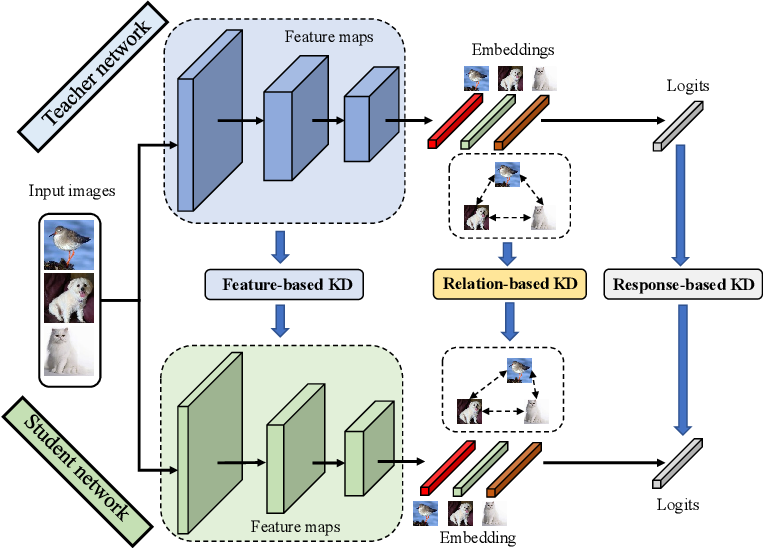
\includegraphics[width=0.88\linewidth]{figures/bcg/KD-M.png}
    \caption{Schematic comparison of response-based and intermediate representation distillation.
             In response-based distillation (left), only the final output of the teacher guides the
             student. In feature-based distillation (right), intermediate activation maps at selected
             layers are additionally aligned via a regression loss. A learnable projector $r_\phi$ is
             employed when the teacher and student feature dimensions are incompatible.}
    \label{fig:kd_paradigms}
\end{figure}

The selection of which layers to use for hint supervision is a non-trivial design decision.
Deeper layers tend to encode more semantically abstract features that are task-specific, while shallower
layers retain more generic, low-level visual information.
In practice, layer selection is often guided by architectural symmetry, cross-validation, or information-
theoretic criteria \cite{heo2019comprehensive}.
The combined training objective integrates both paradigms,

\begin{equation}
    \mathcal{L}_{\mathrm{total}} = \mathcal{L}_{\mathrm{task}} + \lambda_1 \mathcal{L}_{\mathrm{resp}} + \lambda_2 \mathcal{L}_{\mathrm{hint}},
    \label{eq:total_kd_loss}
\end{equation}

\noindent where $\lambda_1, \lambda_2 \geq 0$ are weighting hyperparameters balancing task performance,
output matching, and representational alignment.

% ─────────────────────────────────────────────────────────────────────────────
\section{Diffusion Model Distillation}
\label{sec:kd_diffusion}
% ─────────────────────────────────────────────────────────────────────────────

The application of knowledge distillation to diffusion models is motivated primarily by the high
computational cost of iterative sampling.
Standard Denoising Diffusion Probabilistic Models (DDPMs) \cite{ho2020denoising} require on the order
of $T \sim 1000$ sequential network function evaluations (NFEs) to generate a single sample, as the
reverse process progressively denoises a Gaussian variable $\mathbf{x}_T \sim \mathcal{N}(\mathbf{0},
\mathbf{I})$ through a learned Markov chain.
While accelerated samplers such as DDIM \cite{song2021denoising} and DPM-Solver \cite{lu2022dpm} reduce
the required NFEs to tens or dozens by exploiting deterministic or higher-order ODE integration,
further reduction to a handful of steps—or ideally a single step—without material quality degradation
requires a fundamentally different approach: distillation of the multi-step sampling trajectory into a
student that directly learns to approximate the full trajectory mapping.

\textbf{Progressive Distillation.}
Salimans and Ho \cite{salimans2022progressive} introduced Progressive Distillation (PD) as a response-
based distillation scheme applied iteratively to the diffusion sampling trajectory.
Given a teacher that executes $N$ denoising steps, the student is trained to match the teacher's
\emph{two-step} output in a \emph{single} step, effectively halving the number of required NFEs.
This procedure is applied repeatedly: the trained student is promoted to the teacher role, and a new
student is distilled with another 2$\times$ reduction, yielding a sequence of models requiring
$N, N/2, N/4, \ldots$ steps respectively.
The student's denoising network $\epsilon_\theta$ is trained under

\begin{equation}
    \mathcal{L}_{\mathrm{PD}} = \mathbb{E}_{t, \mathbf{x}_0, \boldsymbol{\epsilon}}\!\left[\omega(t) \left\| \hat{\mathbf{x}}_0^{\mathcal{T}}(\mathbf{x}_t) - \hat{\mathbf{x}}_0^{\mathcal{S}}(\mathbf{x}_t) \right\|_2^2\right],
    \label{eq:progressive_distillation}
\end{equation}

\noindent where $\hat{\mathbf{x}}_0^{\mathcal{T}}(\mathbf{x}_t)$ is the teacher's two-step prediction
of the clean image from the noisy input $\mathbf{x}_t$, $\hat{\mathbf{x}}_0^{\mathcal{S}}(\mathbf{x}_t)$
is the student's single-step prediction, and $\omega(t)$ is a time-step-dependent weighting function.
Progressive Distillation has demonstrated that image quality competitive with the teacher can be achieved
with as few as 4 NFEs, representing an over two-orders-of-magnitude reduction relative to the original
DDPM schedule.

\textbf{Consistency Distillation and Consistency Models.}
Song et al.\ \cite{song2023consistency} proposed Consistency Models, which are grounded in the
observation that all points along a deterministic probability flow ODE trajectory, conditioned on the same
final sample $\mathbf{x}_0$, must be mapped to the same clean image by the learned consistency function
$f_\theta(\mathbf{x}_t, t) \approx \mathbf{x}_0$.
Consistency Distillation (CD) trains the student by enforcing \emph{self-consistency} of adjacent
trajectory points: for two time steps $t > s$ connected by one step of the numerical ODE solver,

\begin{equation}
    \mathcal{L}_{\mathrm{CD}}(\theta, \theta^{-}) = \mathbb{E}_{t, \mathbf{x}_0}\!\left[\, d\!\left(f_\theta(\mathbf{x}_t,\, t),\; f_{\theta^{-}}(\hat{\mathbf{x}}_s,\, s)\right)\right],
    \label{eq:consistency_distillation}
\end{equation}

\noindent where $\hat{\mathbf{x}}_s$ is the one-step numerical estimate of $\mathbf{x}_s$ obtained from
$\mathbf{x}_t$ via a pre-trained diffusion teacher, $\theta^{-}$ are exponential moving average (EMA)
parameters used as the target network to stabilise training, and $d(\cdot, \cdot)$ is a
perceptual or $\ell_2$ distance metric.
Importantly, Consistency Models can also be trained in a teacher-free regime—Consistency Training
(CT)—by bootstrapping the target from the model's own EMA parameters, thus circumventing the need for a
pre-trained diffusion teacher altogether.

\textbf{Latent Consistency Models.}
Luo et al.\ \cite{luo2023lcm} extended the consistency distillation framework to the latent space of
pre-trained latent diffusion models (LDMs) \cite{rombach2022latent}, yielding Latent Consistency Models
(LCMs).
By operating in the compressed latent space of a variational autoencoder rather than in pixel space,
LCMs inherit both the high fidelity of LDMs and the inference efficiency of consistency distillation,
achieving competitive image quality with as few as 2–4 denoising steps on large-scale text-to-image
benchmarks.

The distillation methods described above share a common structural blueprint: a pre-trained diffusion
model serves as the teacher, providing trajectory or output supervision; a student of equal or smaller
capacity is trained to replicate this supervision in fewer function evaluations; and the quality of the
resulting student is evaluated via established metrics such as the Fréchet Inception Distance (FID)
\cite{heusel2017gans} and CLIP score \cite{radford2021learning}.
The specific choice of distillation paradigm—response-based trajectory matching, consistency
enforcement, or adversarial refinement via score distillation sampling \cite{poole2022dreamfusion}—
introduces distinct trade-offs between sample quality, training stability, and generality that will be
examined in depth in Chapter~\ref{chap:knowledge_distillation}.

\begin{figure}[ht]
    \centering
    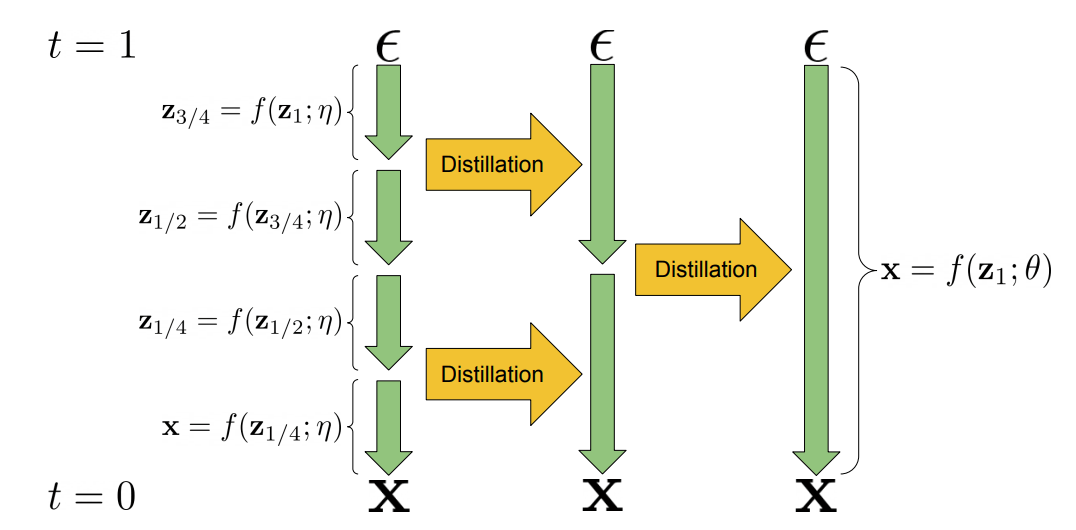
\includegraphics[width=0.92\linewidth]{figures/bcg/progressive_distillation.png}
    \caption{Conceptual overview of diffusion model distillation approaches.
             Progressive Distillation (top) iteratively halves the number of required sampling steps
             by matching two-step teacher outputs with single-step student predictions.
             Consistency Distillation (bottom) enforces self-consistency of all trajectory points
             mapping to the same clean sample $\mathbf{x}_0$, enabling one- or few-step generation.}
    \label{fig:diffusion_distillation_overview}
\end{figure}
\end{figure}